\RequirePackage[l2tabu, orthodox]{nag}
%\documentclass[onecolumn,draft]{svjour3}
%\documentclass[onecolumn,final]{svjour3}
\documentclass[smallextended,final]{svjour3}

\usepackage{amsmath}
\usepackage[round]{natbib}
\usepackage{booktabs}
\usepackage{graphicx}
\usepackage{microtype} % Finetunes spacing, load after fonts
\usepackage{siunitx}
\usepackage{alltt}
\usepackage{wrapfig}
\usepackage[colorlinks=false, pdfborder={0 0 0}]{hyperref} % Should be loaded last
\usepackage[usenames,dvipsnames,svgnames,table]{xcolor}
\usepackage{subfigure}
\newcommand{\nd}[2]{\frac{\mathrm{d} #1}{\mathrm{d} #2}}
\newcommand{\e}{\mathrm{e}}
\newcommand{\tn}{\newline}

\smartqed


\begin{document}

\title{Gentoo Package Dependencies over Time}
\subtitle{Subtitle}
\dedication{}
\author{Remco Bloemen \and Chintan Amrit}
\institute{University of Twente}

\maketitle

\tableofcontents

\begin{abstract}
Open source distributions such as Gentoo need to accurately track dependency relations between software packages in order to install working systems. To do this, Gentoo has a carefully authored database containing those relations. In this paper, we extract the Gentoo package dependency graph and its changes over time. The final dependency graph spans 15 thousand open source projects and 80 thousand dependency relations. Furthermore, the development of this graph is tracked over time from the beginning of the Gentoo project in 2000 to the first quarter of 2012, with monthly resolution. The resulting dataset provides many opportunities for research. In this paper we explore cluster analysis to reveals meaningful relations between packages and in a separate paper we analyze changes in the dependencies over time to get insights in the innovation dynamics of open source software.
\end{abstract}


\section{Introduction}

We study software innovation from the adoption perspective. Adoption reflects innovation 'better' than changes within packages. Because reasons.

\begin{figure}
\centering
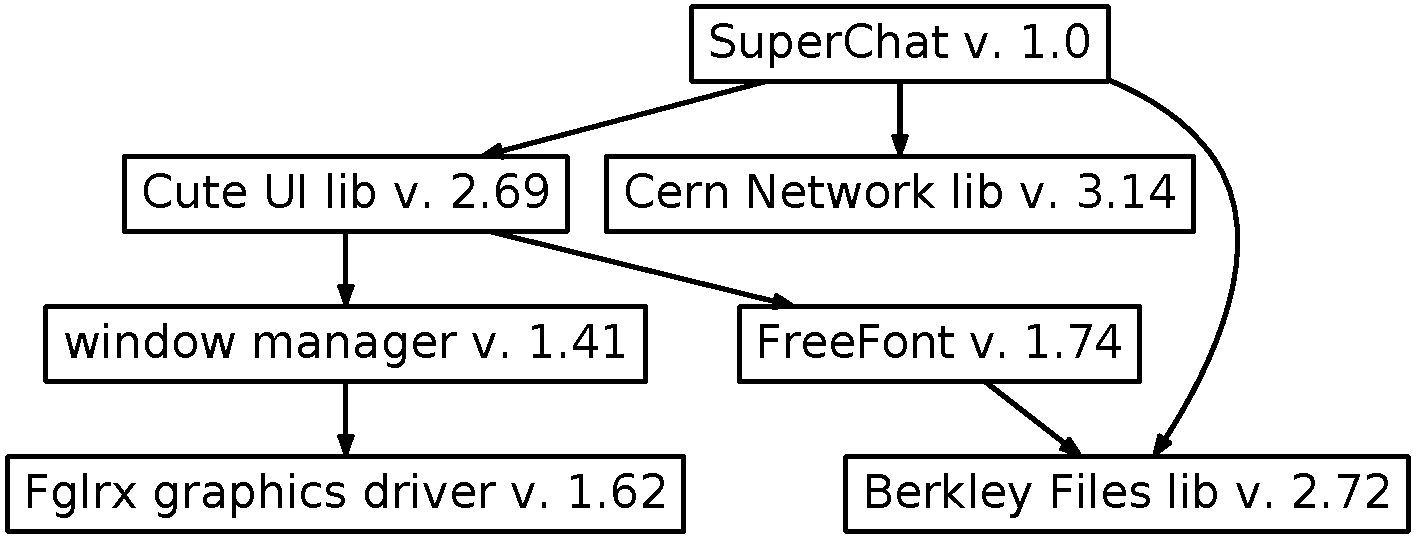
\includegraphics[width=\linewidth]{depgraph.pdf}
\caption{Example dependency graph.}\label{fig:depgraph-chat}
\vspace{-1em}
\end{figure}

No software project stands entirely on its own. Software is usually developed by taking one or more existing libraries of components and combining those components in ways to create new products. Take for example a simple chat application. The chat application uses a different library for user interface development that provides components such as a window a text entry field and a button (that is labeled "send message" by the chat application). This user interface library in its turn uses a graphics library to draw the lines, rectangles and text necessary for the fields and buttons. The graphics library uses a library to read font files and uses the fonts to turn text into pictures that can be displayed on the screen. The graphics library then sends the contents of the window to the window manager, which in turns uses a graphics card driver to instruct the hardware. The chat application uses a networking library to provide it with the basic components for internet communication and uses a file library to store the users settings. The same file library is also used by the font library to read font files. The dependency graph so described is drawn in figure~\ref{fig:depgraph-chat}. Compared to a real chat application the graph is hugely simplified, tracing a real chat application back to all the components involved will likely result in hundreds of libraries used.

In the remainder of this article, the terms `project', `package' and `library' will be used as synonyms for a node in the dependency graph.

Now that a data source is selected, it is time to extract the required information and process the data into a form that allows easy calculations. The major steps are collecting the raw data, parsing this into a simpler format and producing the final dependency graph from this simpler form. Some post-processing can then be done on the dependency graph. In the process, the dataset will shrink from thirteen gigabytes taking more than a week to collect, to thirty megabytes that can be processed in four seconds.

\section{Related work}

In \citet{crowston08} published a comprehensive overview of academical research on open source software development. Of the 184 articles they cite, the vast majority of articles are case studies or surveys, with 4\% of the articles describing the development of empirical instruments and/or measurements. Also, most articles look at the level of a particular group or project, with 4\% looking at the societal level of interacting projects. Crowston et al. find no articles that develop instruments or measurements on the level of OSS packages, which this paper aims to do.

In their 2008 article \citet{zheng08} analyse the dependency graph of the Gentoo Portage package database as it was in February 2007. The global structure of the graph is analysed in graph theoretic terms of sparsity, clustering coefficient, degree distribution and degree growth rate. The authors conclude that the graph can not be explained well by existing models of network growth and they propose two new models instead. Our study differs in two ways: First, we analyse the changes to the dependency graph over time, whereas Zheng et al. look at a particular instance in 2007. Second, we analyse and model the development of a given software package in the dependency network, instead of the overall development of the network. It can be interesting to study how the Bass diffusion model for the development of individual nodes corresponds to Zheng et al. model for the development of the whole graph.

\citet{haefliger08} study code re-use on six open source projects, they conclude that there is extensive code re-use in open source software. The article proceeds by identifying the process of code re-use, such as the drivers for re-using and the tools used to find relevant code. The study by Haefliger et al. looks at a given project and how it  re-uses existing components, whereas this paper looks at a given project and how it is being re-used by other projects. Additionally, we performed our analysis using a large set of automatically collected and processed empirical data.

\citet{dedrick04} and \citet{chen06} study the adoption process of open source software by (commercial) end users. Their focus is on the competitive economic strengths of open source software versus commercial software. The conclusion is that cost is the most important driver for open source adoption and freedom and extensibility plays a lesser role. The articles do not provide empirical data on the adoption process itself, which makes it hard to compare it to our present finding of a Bass diffusion adoption process.


Why this order?

\subsection{Innovation theory}


\subsection{Software innovation}

→ Look for review papers on software innovation and software adoption


\subsection{Innovation theoretic models of adoption}


\subsection{Innovative adoption in software}


\subsection{Software package dependencies}

European research project 2008—2011 aiming to ``solve the upgrade problem''.
EDOS project

http://www.mancoosi.org/papers/

Boender 

The Ultimate Debian Database: Consolidating bazaar metadata for Quality Assurance and data mining
Full Text Sign-In or Purchase
2 Author(s)
Nussbaum, L. ; LORIA, Nancy-Univ., Nancy, France ; Zacchiroli, S.

German et al. The Evolution of the R Software Ecosystem

Mining Challenge 2010: FreeBSD, GNOME Desktop and Debian/Ubuntu


Life and death of software packages: an evolutionary study of Debian
Raymond Nguyen  University of Waterloo, Waterloo, Canada
Ric Holt        University of Waterloo, Waterloo, Canada


Research question:

* The authors do not seem to be aware of the large body of research on dependencies between components. For instance, it is not clear why does one need to design a new text-based formal for inter-package dependencies while Common Upgradeability Description Format, CUDF [http://www.mancoosi.org/reports/tr3.pdf], has been proposed by Treinen and Zacchiroli more than five years ago. Numerous papers have analysed data in the CUDF format, and yearly MICS (Mancoosi International Solver Competition) have been organized in 2010, 2011 and 2012. Additional papers published as part of the Mancoosi project are available on the project site: http://www.mancoosi.org/ For more recent work on upgrade dependencies the authors might consult a paper by Schoenmakers et al. [WCRE 2013].

Power law distributions:

A. Clauset, C.R. Shalizi, and M.E.J. Newman, "Power-law distributions in empirical data" SIAM Review 51(4), 661-703 (2009).

\subsection{Innovation diffusion}

\emph{Diffusion} is the process of market uptake of an innovation, the users of a particular innovation are called \emph{adopters} \citep{narayanan01}. Taking the open source projects as a 'market', these concepts can be applied to libraries and dependencies. For example, consider the projects with a graphical user interface (GUI). These have a demand for a GUI toolkit, and there are several competing implementations available (\verb|Qt|, \verb|GTK|, \verb|Wx|, etc..). The introduction and uptake of a new GUI toolkit is a process of innovation diffusion and the projects that use a particular toolkit can be considered adopters of that toolkit. When talking about software projects such a relation is often called a \emph{dependency}.
In the next section we describe the Bass \citep{bass69}  diffusion model, we then describe the results of our analysis of fitting the Bass diffusion model on the Gentoo portage package dependency graph. This is followed by a discussion of the results of our analysis and finally we end the paper with the conclusions from our analysis and some discussion of possible future work.



\subsection{The Bass diffusion model}\label{sect:Bass}

Once an innovation is released to the public a process starts where an increasing portion of the market decides to use the innovation. In the theory of innovation dynamics this process is called diffusion and the users are called adopters. \citep[see][chapter 4]{narayanan01}

To model the process of innovation diffusion \cite{bass69} introduces two processes that propagate an innovation. The first processes is involves individuals that decide to use an innovation based on their perception of its merits, without looking at the experiences of others. The second process involves the word-of-mouth effect or the bandwagon effect, individuals adopt the innovation solely because they hear of the experiences of previous adopters. Of course in reality, everyone will be somewhere in between these two extreme types, but for the sake of modelling it suffices to consider the relative abundance of both types.

It should be noted that \cite{bass69} and all later authors, use confusing terms to describe the two types of adopters. The first type are called "innovators", not to be confused with those actually inventing the innovation and the second type are called "imitators", not to be confused with those developing imitating offerings. If one remembers that the model concerns the demand side of the market and not the supply side than it will all be clear.

To model the diffusion process, let $M$ be the total market size for the innovation and $A$ the current number of adopters, such that $0 \ge A \ge M$. The two adoption processes can then be described as follows: \citep[see also][]{bass10,mahajan90}

\emph{Innovators}: Some individuals in the market that don't use the innovation might decide to adopt the innovation. The rate at which this happens is $p$, the coefficient of innovation. The number of user that do not use the innovation is $M-A$, so the inflow of adopters is $p(M-A)$.

\emph{Imitators}: The people who use the innovation can express their fondness to people who do not yet use the innovation, which can influence them to adopt the innovation. The rate at which this happens is $q$, the rate of imitation. The number of user that do not use the innovation is again $M-A$, the chance of meeting someone that does use the innovation is proportional to $\frac{A}{M}$ so the inflow of imitators can be modelled as $q\frac{A}{M}(M-A)$.

When these two effects are combined, the net inflow of users, represented by the time derivative of $A$, can be modelled as:
\begin{align*}
\nd{A}{t} &= p(M - A) + q\frac{A}{M}(M - A) \\
&= \left(p + q\frac{A}{M} \right)(M - A)
\end{align*}

Often one is not concerned with the market size $M$ and only interested in the fraction of the market---denoted with $F$---that uses the innovation. Of course, $F=\frac{A}{M}$. By dividing the above equation with $M$ one obtains the Bass model:

\begin{align}\label{eq:bass-ode}
\nd{F}{t} &= \left(p + q F\right)(1 - F)
\end{align}

\cite{bass69} solves this ordinary differential equation, which results in the following function for $F$:

\begin{align}\label{eq:bass-direct}
F(t) &= \frac{1 - \e^{-(p+q)t}}{1+\frac{q}{p}\e^{-(p+q)t}}
\end{align}

\begin{figure}\small\centering
\caption[Bass model of innovation diffusion]{The Bass model of innovation diffusion. The blue trace represents a Bass diffusion with $p=0.01$ and $q=0.90$. The purple trace bass diffusion with $p=0.90$ and $q=0.01$.}
\label{fig:bass}
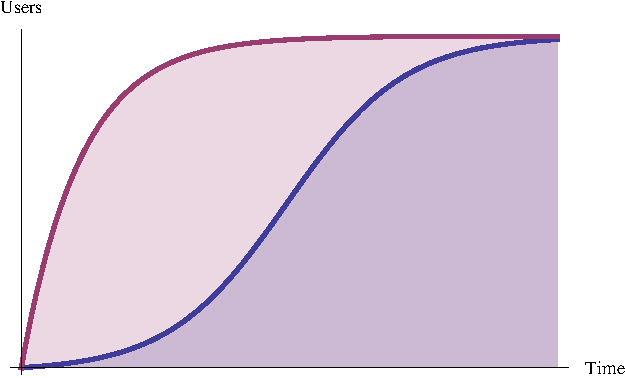
\includegraphics{Bass.pdf}
\end{figure}

In figure~\ref{fig:bass} two Bass diffusions are plotted using equation \eqref{eq:bass-direct}, one representing an innovation diffusion with many innovators and few imitators and one representing a diffusion with many imitators and few innovators. When there are more imitators it takes a while for the innovation to take of since the majority of the potential users are waiting for someone else to try it first.

To fit the model of equation~\eqref{eq:bass-direct} to empirical data two additions are necessary. First the market size has to be re-introduced, this is done by taking $A(t) = M F(t)$. The market size, $M$, in this equation represents the total number of potential adopters for this specific product, not the total number of adopters for a category of products. Since it is not possible to know in advance who will eventually be using an innovation it is difficult to determine $M$ in advance. Furthermore, the Bass model assumes the market size to be constant and competition free, which is unlikely in practise. Therefore the quantity has to be fitted to the data, statistical goodness-of-fit measures can then be used to determine the validity of the assumptions. The second addition is the time at which the innovation is introduced. Until now the assumption was that the introduction was at $t=0$, in arbitrary units. For empirical data fitting it is necessary to be able to specify an arbitrary introduction time. This can be achieved by introducing the introduction time $t_0$ in the equation as $A(t) = M F(t - t_0)$. Again, this variable can be fitted if it can not be determined in advance.

\begin{align} \label{eq:bass-model}
	A(t) &= M \frac{1 - \e^{-(p+q)(t-t_0)}}{1 + \frac{q}{p}\e^{-(p+q)(t-t_0)}}
\end{align}

Equation~\eqref{eq:bass-model} incorporates the two additions and can be readily applied to empirical data. In \cite{mahajan95} and many other empirical studies this happens in the differential form, since only absolute sales figures are available and not absolute user figures. The dependency graph method presented later allows one to obtain absolute usage number, so the differential form is not further used. 


The interpretation of the variables and parameters and their dimensions is presented in table~\ref{tbl:bass-model}. When applying the formula one should note that it is non-linear, so ordinary linear regression can not be used. Instead one can use non-linear least squares regression, but note the correct number of the degrees of freedom. This can be done using existing mathematical/statistical packages. For this thesis the  \verb|NonlinearModelFit| procedure in Mathematica was used. 

\begin{table}\centering\small
\caption[Bass model variables and parameters]{Overview of the variables and parameters of the Bass model as presented in equation~\eqref{eq:bass-model}.}
\label{tbl:bass-model}
\begin{tabular}{cll}
\toprule
& Dimension & description \\
\midrule
$A$   & adopters    & adopters at a the model time \\
$t$   & time        & model time \\
\midrule
$t_0$ & time        & time of innovation introduction \\
$M$   & adopters    & number of potential adopters \\
$p$   & time$^{-1}$ & rate of adopter innovation \\
$q$   & time$^{-1}$ & rate of adopter imitation \\
\bottomrule
\end{tabular}
\end{table}

To model the process of innovation diffusion, Bass \citep{bass69} introduces two processes that propagate an innovation. The first processes involves individuals that decide to use an innovation based on their perception of its merits. The second process involves the word-of-mouth effect or the bandwagon effect: individuals adopt the innovation because they hear of the experiences of previous adopters. In reality however, everyone will be somewhere in between these two extreme types, but for the sake of modelling it suffices to consider the relative contribution of both types. It should be noted that for historical reasons \citet{bass69} and all later authors use the following terms; the first type are called "innovators", not to be confused with those actually inventing the innovation and the second type are called "imitators", not to be confused with those developing imitating offerings. Taking $M$ to stand for the total market size and $A$ to stand for the total number of adopters the Bass diffusion can be modelled with two simultaneous processes:

\emph{Innovators}: Market participants not using use the innovation yet might decide to adopt the innovation. The rate at which this happens is $p$, the coefficient of innovation. The number of user that do not use the innovation is $M-A$, so the inflow of adopters is $p(M-A)$.

\emph{Imitators}: Users of the innovation can express their fondness to market participants who do not yet use the innovation. This can influence them to adopt the innovation at a rate $q$, the rate of imitation. The number of user that do not use the innovation is again $M-A$, the chance of meeting someone that does use the innovation is proportional to $\frac{A}{M}$ so the inflow of imitators can be modelled as $q\frac{A}{M}(M-A)$.

When these two effects are combined the net inflow of adopters represented by the time derivative of $A$ can be modelled as

\begin{align}
	\nd{A}{t} &= p (M-A) + q\frac{A}{M}(M-A) \text{.}
\end{align}

This first order homogeneous ordinary differential equation can be solved for $A(t)$ to give

\begin{align} \label{eq:bass}
	A(t) &= M \frac{1 - \e^{-(p+q)t}}{1 + \frac{q}{p} \e^{-(p+q)t}} \text{.}
\end{align}

The solution assumes the innovation is introduced at time zero, to account for this the substitution $t \rightarrow t - t_0$ is made. This results in four parameters, $t_0$, $M$, $p$ and $q$ that can be fit to the empirical data.




\section{The Gentoo Portage Dataset}

The empirical data used is the time evolution of the Gentoo Portage package dependency graph \citep{rem14}. This dataset contains the full dependency graph for every month since the project was initiated in $2000$, the resulting graphs have a combined total of 1.3 million packages and 6.9 million dependency relations, with the largest graph having 15 thousand packages and 80 thousand dependency relations.

Special tools where developed to extract the time series of the number of adopters $A_t$ for a given package. This time series was then fit to \eqref{eq:bass} using Mathematica's \texttt{NonLinearModelFit}. The goodness-of-fit was analysed using an ANOVA table and calculated using the adjust coefficient of determination $\bar{R}^2$. The parameters were extracted from the fit, and confidence intervals were calculated under assumptions of normality. In \ref{tbl:results} the relevant parameters are presented with their mean value and a $95\%$ confidence interval. Since normality was assumed, the confidence intervals ignore the $p \ge 0$ and $q \ge 0$ constraints. 

The plots were drawn using a thick red line for the model and shades of red for the prediction bands. The thick red line was drawn according to \eqref{eq:bass}, with the mean values used as parameters. Then single value predictions bands were calculated for $90\%$, $95\%$, $99\%$ and $99.9\%$ confidence and were drawn in progressively darker shades of pink. They represent a prediction for where a single additional value would likely fall. According to the model and the uncertainty introduced by the fit, there is a $90\%$ chance that it will fall in the innermost band, $95\%$ chance that it would falil in the second band, etc. If the data fits the model properly, one would expect to see $90\%$ of the points in the inner band. Finally, the empirical data points were plotted as black dots, connected with a thin vertical line - the residual error of the model.


\subsection{Collecting}

The Gentoo portage database consists of a large number of text files, at least one for every version of every package, contained in a large directory structure. This entire structure is kept in a CVS revision control system that has tracked all changes to the database since the start of the project around 2000.

Using the \verb|cvs| command one can download the entire database as it was at a certain point in history. For example the following command would download the database, as it was on 1 December 2003:

\begin{verbatim}
cvs -d :pserver:anonymous@anoncvs.gentoo.org\
  /var/cvsroot co -D 12/01/2003 gentoo-x86
\end{verbatim}

Using a small utility written for the task, this command was repeatedly invoked to download all the databases from 1 January 2000 until mid 2012, with increments of one month. The \verb|.ebuild|, \verb|.eclass| and \verb|.eblit| files are stored. Other files are ignored, to save space since they contain no relevant information. This whole downloading processes took about a week and a half and the resulting database consists of three million files occupying thirteen gigabytes of space. There are also files specifying packages renames, but since these only get appended to and never deleted they where taken from the latest version of the database.

\subsection{Parsing}

The files are written in a text based computer language called `ebuild' which is based on the Bash shell script language. Being a scripting language, the files can refer to other files and include complicated code to calculate dependencies on demand. This eases the task of the script developer, since he can automate many processes, but it complicates the task of extracting data. Several approaches where tried to extract the data in the industrial quantities the analysis requires.

The first approach was to use Paludis and its C++ bindings to load a repository and extract metadata. Paludis is a tool designed to process ebuild files, we then query its database interface to gather all the dependency information from all the packages. This approach takes a lot of time, it requires around a half an hour per database version, but it fails on some of the older databases because the format of the database changed over time.

% Eclasses
The second attempt was to use a custom build metadata extraction program that also supports an older version of the database. This parser looks for text patterns resembling dependency specifications and implements only a minimal amount of the ebuild file format (basically only dependencies and the \verb|inherit| inclusion statement). This technique is very fast, processing the entire set in 70 minutes, but fails on the newer databases that use complex techniques such as macro's in the dependency specifications.

The final method is a hybrid of the first two, using the Paludis' \verb|instruo| command to pre-process and expand all the macros to create simplified versions that can be parsed using the custom parser. The \verb|instruo| command was run on every version of the database downloaded. Where the command failed on a package (the older format ones) the original was kept. The total running time of this operation was around four days.

\subsection{Producing the Dependency Graphs}

Now the data is in 154 snapshots of the package database in a simplified text based format. This is several gigabytes and several millions of files large and needs to be processed into dependency graphs. Obviously it is inhumane to do this by hand, therefore more specialized tools were developed.

\begin{figure}[t]
\begin{alltt}
>=media-libs/taglib-1.6.1[asf,mp4]
>=media-libs/taglib-extras-1.0.1
player? (
    app-crypt/qca:2
    >=app-misc/strigi-0.5.7[dbus,qt4]
    || ( >=dev-db/mysql-5.0.76
         =virtual/mysql-5.1 )
    >=kde-base/kdelibs-4.3[opengl?,semantic-desktop?]
    sys-libs/zlib
    x11-libs/qt-script
    >=x11-libs/qtscriptgenerator-0.1.0
\end{alltt}
\vspace{-1em}
\caption{Fragment of the runtime dependencies of the Amarok music player.}\label{fig:amarokruntime}
\vspace{-2em}
\end{figure}

By design the database can work with complicated dependency relations, such as ``package \verb|amarok| requires package \verb|phonon-kde|, minimum version \verb|4.3|, but only when feature \verb|player| is required''. This is would be coded as \verb|player?| \verb|(| \verb|>=kde-base/phonon-kde-4.3| \verb|)|. An example of the run time dependencies for the Amarok music player is given in figure~\ref{fig:amarokruntime}. The figure includes more complex rules such as ``either package X or package Y is required'', `` package X is required to contain feature Y'', etcetera.

% Ignoring version specifiers, conditionals, blocks, use flags
These conditional rules are relevant when compiling and running software, but the conditions are not necessary when analysing component use from an innovation perspective. If Amarok has an optional dependency on a package, the developers of Amarok are actively using the innovation provided by that package even though it may not be enabled by the end user in the final product. For this reason, and of simplicity, all the conditionals are ignored when parsing the ebuilds.

% Only process latest version at the time of the snapshot
When a database snapshot contains several versions of the same package, only the latest is used. For some of the analysis techniques presented in the version information might be relevant, but at this point it was decided not to include different versions to simplify processing analysis. When several versions where available in the database at a certain point in time, only the highest version was included. This ensures that each snapshot represents the state of art at that time.

% Parsing DEPENDS, RDEPENDS and PDEPENDS
In the Gentoo Portage database the dependencies are sorted in two kinds, compile time dependencies and runtime dependencies. The first kind are required to build and install the package. The second kind is only required when actually using the package. The reason for this distinction is a technical: it solves installation issues with cyclical dependencies. For the current purposes both kinds of dependencies are considered equal.

% Package moves
Sometimes, package get renamed or moved around in the database, this needs to be accounted for. Luckily, to allow users to upgrade from an older version to a newer version the processing of moves and renames has been automated in the Gentoo Portage database. The developers maintain a list of all the moves and renames that have happened in the database in a structured format. The latest version of this list is used to retroactively change all the package names in the historical snapshots to their modern name. This ensures that moves and renames do not harm historical continuity in the dataset.

% Package provides
Using all the observations and choices made above, a tool was developed to extract dependency graphs from all the simplified database snapshots. The shear scale of the resulting dataset, $1.3$ million packages and $6.9$ million dependency relations, required a solution to store efficiently. Therefore, a compressed format was developed that only stores the changes between the historical snapshots instead of storing whole snapshots. The extraction process took three hours and resulted in a $29$ megabyte file. Reading this file into memory resident data structures and performing simple queries takes about $4$ seconds. The dataset is now in a usable form.

\subsection{Final Remarks}

The dataset collected is available at
\\\url{http://datahub.io/dataset/gentoo-dependency-graph}\\
as compressed GML graphs for every snapshot. Raw data is available at
\\\texttt{http://www.utwente.nl/mb/iebis/staff/amrit/}\\\texttt{timeline.squashfs}\\
as a SquashFS compressed filesystem. The SquashFS format allows one to mount the compressed data as a read-only disk drive and operate directly on the dataset. It contains the pre-processed ebuild files and the file \verb|graphs.bip| that contains all of the graphs in a custom format specialized for quick processing of large graphs over time. A C++ toolkit to work with the \verb|graphs.bip| file is available at \url{https://github.com/Recmo/depgraph}.

In a separate paper \citep{rem142} we analyzed the changes in the dependency graph over time. In particular the growth of the number of dependers on a given package is explained using the Bass model of innovation diffusion.

\begin{table}
\centering
\caption{Key figures of the dataset}\label{tbl:dataset}
\begin{tabular}{ll}
\toprule
\multicolumn{2}{c}{\emph{Time}} \\[0.5mm]
Period & 2000 to Q1 2012 \\
Resolution & Monthly \\
Snapshots & 154 Graphs \\
\midrule
\multicolumn{2}{c}{\emph{All graphs}} \\[0.5mm]
Nodes & 1.3 Million \\
Vertices & 6.9 Million \\
\midrule
\multicolumn{2}{c}{\emph{Final graph}} \\[0.5mm]
Nodes & 15 Thousand \\
Vertices & 80 Thousand \\
\midrule
\multicolumn{2}{c}{\emph{Raw ebuilds}} \\[0.5mm]
Format & SquashFS \\
Size & 239 MB (compressed) \\
 & 4.4 GB (uncompressed) \\
Files & 2,990,722 \\
\midrule
\multicolumn{2}{c}{\emph{Compressed graphs}} \\[0.5mm]
Format & Tar+XZ compressed GML \\
Size & 2 MB \\
\bottomrule
\end{tabular}
\end{table}



\section{Exploring the Dataset}


\begin{figure}
\centering
\subfigure[Total number of packages]{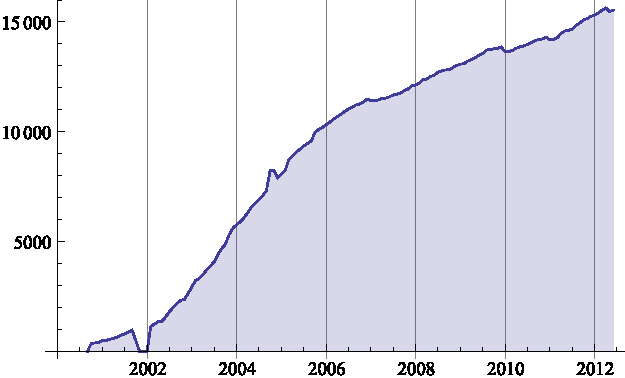
\includegraphics[width=0.45\textwidth]{packageCountUnfiltered2.pdf}\label{fig:pkgsgrowth}}
\subfigure[Additions and removals]{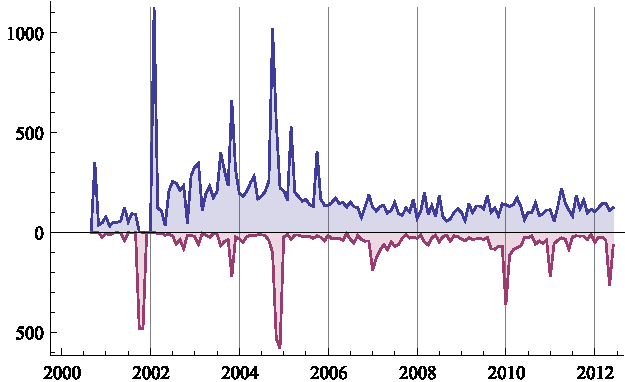
\includegraphics[width=0.45\textwidth]{packageCountDeltaUnfiltered2.pdf}\label{fig:pkgsgrowthdelta}}
\caption{Growth of the Gentoo package database over time.}\label{fig:pkgsgrowth}
\end{figure}

In figure~\ref{fig:pkgsgrowth} the number of packages in the database is plotted over time. One can see how the database started in 2001, underwent a period of rapid growth between 2002---2006 and settled into calm a linear growth from 2006 onwards. In figure~\ref{fig:pkgsgrowthdelta} the rate of introducing and removing packages is plotted over time. This show two spikes, one at the start of 2002 and one in 2005. The cause of these spikes was not thoroughly investigated, but a likely cause is a massive cleanup and refactoring of the database. This is a warning sign that the data exactly at these points might contain a lot of noise. In general, the data before 2006 should be considered with more caution than the data afterwards.

The effect of the growth of the entire dataset on the number of dependencies for individual packages was investigated, but no influence was found. Since the total number of packages grows one would expect the `market' for a certain package to grow and thus the number of dependency relations to that package to grow. To compensate for this one could divide the number of dependers by the total number of packages, compare this with using a market-share instead of an absolute number of users. In practice, this only made any significant difference for early data, but that was determined to be unreliable anyway. In the interest of keeping the analysis simple no compensation was made for the growth of the number of packages.

One of the first thing attempted after generating the dataset was to visualize the entire graph of the latest snapshot. The problem is, to make any sense of a graph it has to be laid out visually on a plane, nodes that are connected should be placed close to each other so that connecting lines are short and have little overlap. Software packages such as Graphviz, Tulip, Gephi, Jetty and Cytoscope have been tried, but after days of trying and many hours of calculation, none where able to produce any insightful layout for the sixteen thousand nodes and hundred thousand relations.

\begin{figure}
\centering
\subfigure[Dependencies per package]{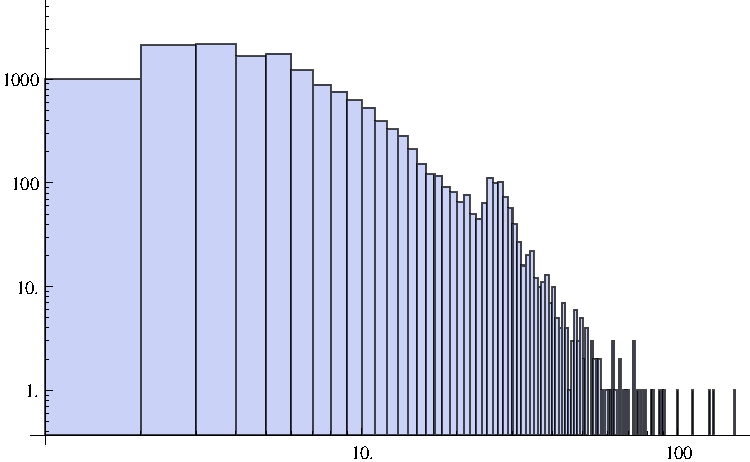
\includegraphics[width=0.45\textwidth]{histo-out.pdf}\label{fig:dephisto-out}}
\subfigure[Dependers per package]{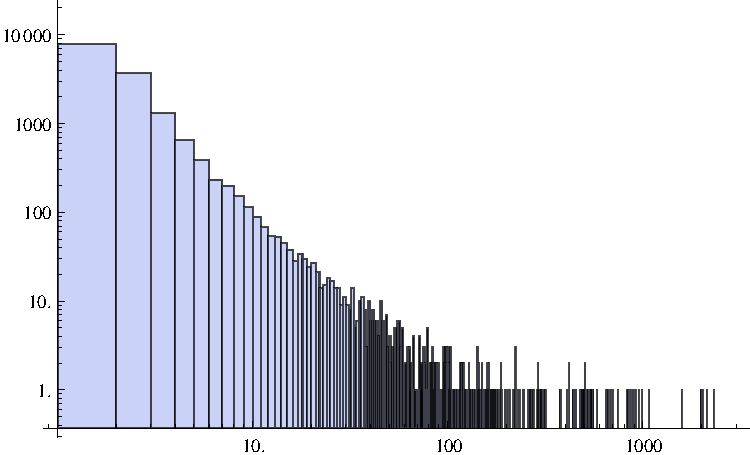
\includegraphics[width=0.45\textwidth]{histo-in.pdf}\label{fig:dephisto-in}}
\caption{Double logarithmic histograms of the number of incoming and outgoing dependencies per package.}
\end{figure}

Since it was impossible to get a visual overview of the entire dependency graph, its structure was plotted using histograms. Figure~\ref{fig:dephisto-out} is a histogram of the number of dependencies per package. A log-log scale was required to make the plot insightful, this reflects the fact that there are many packages with only zero, one or a few dependencies and a few packages with a lot of dependencies. Statistically this means the distribution of the number of dependencies has a fat tail. Likewise, the number of dependers for each package is plotted in figure~\ref{fig:dephisto-in}. This can be interpreted as the distribution of the number of adopters of a given technology. Again, there is a fat tail, even fatter than the one from the number of dependencies. The approximate linearity of the histogram suggest a power-law like distribution of the number of adopters for a given technology. \citet{zheng08} suggest that the structure of package dependency networks is not comparable to known models of social networks and have developed their own model to explain the graph structure.

Since it was impossible to get a visual overview of the entire dependency graph, its structure was plotted using double logarithmic histograms. It was found that there there are many packages with only zero, one or a few dependencies and a few packages with a lot of dependencies. Statistically this means the distribution of the number of dependencies has a fat tail. Likewise, the number of dependers for each package was plotted, this can be interpreted as the distribution of the number of adopters of a given technology. Again, there was a fat tail, even fatter than the one from the number of dependencies. The histogram was approximately linear in the double logarithmic scale, suggesting a power-law like distribution of the number of adopters for a given technology. \citet{zheng08} suggest that the structure of package dependency networks is not comparable to known models of social networks and have developed their own model to explain the graph structure.

\subsection{The KDE Subgraph}

The entire graph might be difficult to visualize, but a small part should be easier. The problem with choosing a small part is that the part must have a meaningful boundary, a random selection will likely have few relations and miss some key packages. It was therefore decided to only pick the packages that belong to the KDE desktop environment. The primary reason is that the author is familiar with this set of packages and knows its structure in some detail. A secondary reason is that the packages are developed by a tightly connected community where component reuse among the projects is stimulated by creating libraries. The selection was implemented by considering only packages in the category \verb|kde-base| from the Gentoo Portage database.

The program Tulip was used to visualize the graph, the result is in figure~\ref{fig:kde2}. First the graph was laid out using a force based method, this clusters packages that are strongly connected close to each other. Then the graphs where colored according to their $k$-core measure, this is a measure for the `connectedness' of a package. At this point there was still an unclear mess of lines between the packages, this was resolved by bundling the edges. Edge bundling merges neighboring lines to a single thicker line, this creates a vein-like structure. 

\begin{figure}
\centering
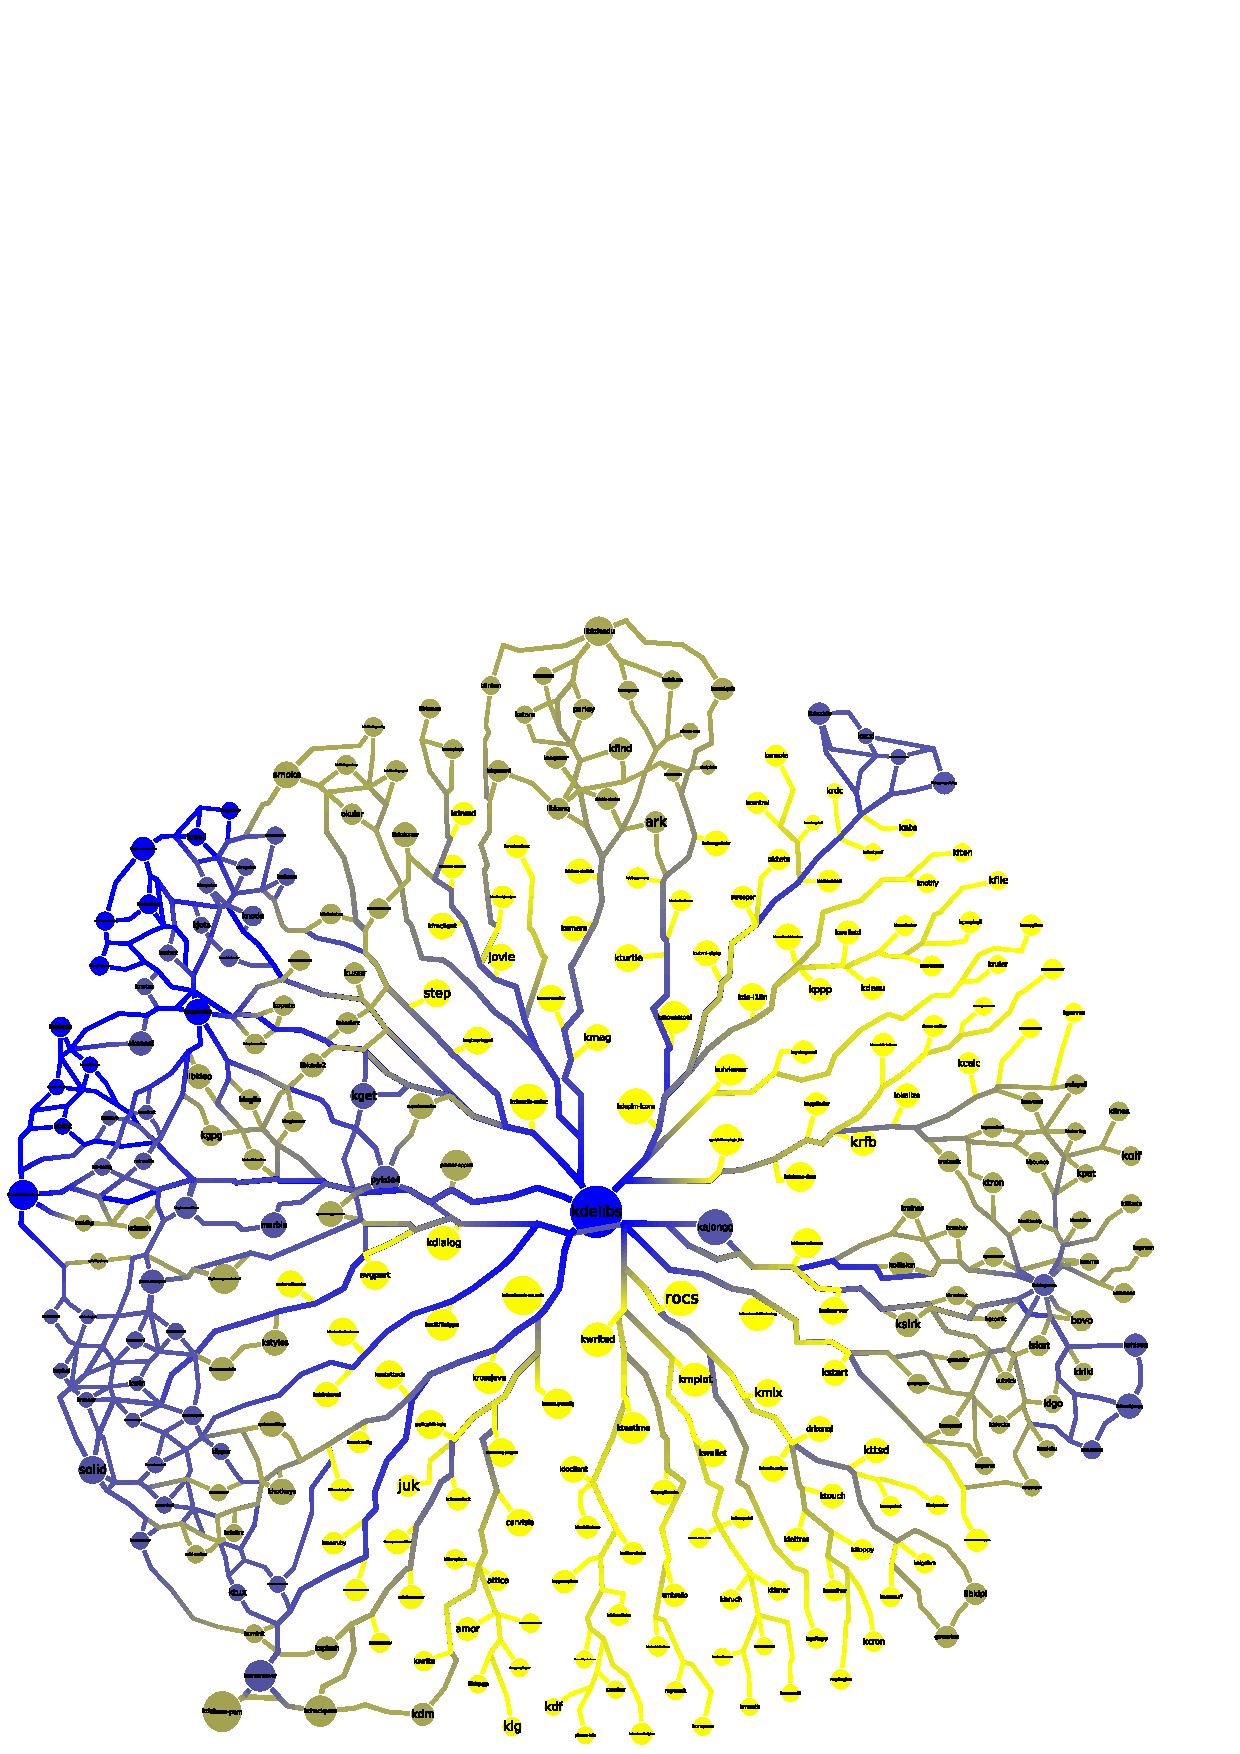
\includegraphics[clip,trim=0 0 1cm 10cm,width=\linewidth]{kde.pdf}
\caption{Internal dependencies of modules in the KDE project. Color represents the $k$-core measure. The graph edges have been bundled to improve readability.}\label{fig:kde2}
\end{figure}

In figure~\ref{fig:kde2} one can see that all the packages depend on \verb|kdelibs|, the large blue dot in the middle. The \verb|kdelibs| package provides a lot of basic functionality, such as a unified set of icons, file open/save dialogues and less visible standard components. Almost all the packages in the KDE set require one or more of these components. It should be stressed that there was no manual work involved in the layout of this graph, Tulip was able to determine using only objective, deterministic mathematical methods from graph theory that \verb|kdelibs| plays a central role in the KDE technology.

The second thing to notice are the clusters that form along the edge of the figure. All these clusters represent related areas of technology within KDE. The brownish-grey cluster immediately at the top contains mostly educational software and a few file utilities. Going clockwise, the little blue cluster next to it contains programs for compact discs. The large brownish-grey cluster on the right consists exclusively of games and supporting technologies. The complex mesh that starts around seven o'clock begins with technology used to allow users to log in. It then proceeds towards hardware related technology and desktop infrastructure. The big blue dot marked `solid' at eight o'clock is KDE's hardware abstraction layer. At nine o'clock the big blue dot represents the notification library, used to notify users of hardware events (``battery low'' and the likes), appointments or incoming emails. The mesh now shifts towards personal information management at ten o'clock. These contain utilities such as an email client, a note taking application, a chat client and a calendar application and related technologies. Lastly, the small brown-grey cluster at eleven o'clock contains technology to allow integration of scripting languages.

Scattered throughout the figure are yellow dots containing packages that are only connected to \verb|kdelibs|, without any apparent pattern in their location. This was expected since the packages only depend on \verb|kdelibs| and are not depended upon by other packages. This means there is no information that brings any insight in their nature and where to cluster them. Perhaps if dependencies from outside the KDE subset where included the packages would form more clusters.

It is remarkable how only a few dependency relations provide sufficient clues for the clustering algorithm to automatically find related areas of technology. Similar but faster clustering techniques where used on the whole snapshot with similar results. Related packages for certain programming languages (Perl, Php, Java, Python, Ruby) would cluster and packages related to either KDE or GNOME would cluster, among many more. Unfortunately the analysis software was struggling with the size of the dataset and the full set was not investigated further.

\section{Results}

From the entire list of packages, a few well-known (at least according to the author) packages where selected. The selection criteria was that the package must not have existed before (around) 2004, because the Gentoo Portage database was still too immature then, and the package must have gained a considerable number of dependers since its introduction. In \ref{tbl:results}, we list some selected packages along with their parameters. In all cases the adjusted coefficient of determination $\bar{R}^2$ was more than $99\%$.

\begin{table}
\centering
\caption{Results of fitting the Bass model.}\label{tbl:results}
\begin{tabular}{lr@{ $\pm$}rr@{ $\pm$}rr@{ $\pm$}r}
\toprule
Package & \multicolumn{2}{c}{$p$} & \multicolumn{2}{c}{$q$} & \multicolumn{2}{c}{$M$} \\
\midrule
\texttt{git}         & 0.00 & 0.01    & 0.73 & 0.13   & 746 & 394 \\
\texttt{libnotify}   & 0.05 & 0.08    & 0.72 & 0.30   & 103 &   9 \\
\texttt{udev}        & 0.01 & 0.01    & 0.50 & 0.12   & 200 &  65 \\
\texttt{cairo}       & 0.01 & 0.01    & 0.43 & 0.09   & 249 &  44 \\
\texttt{libmad}      & 0.18 & 0.14    & 1.13 & 0.3    &  55 &   1 \\
\texttt{libtheora}   & 0.11 & 0.09    & 0.63 & 0.21   &  32 &   1 \\
\texttt{taglib}      & 0.22 & 0.03    & 0.04 & 0.06   &  62 &  12 \\
\bottomrule
\end{tabular}
\end{table}

\begin{figure}
\centering
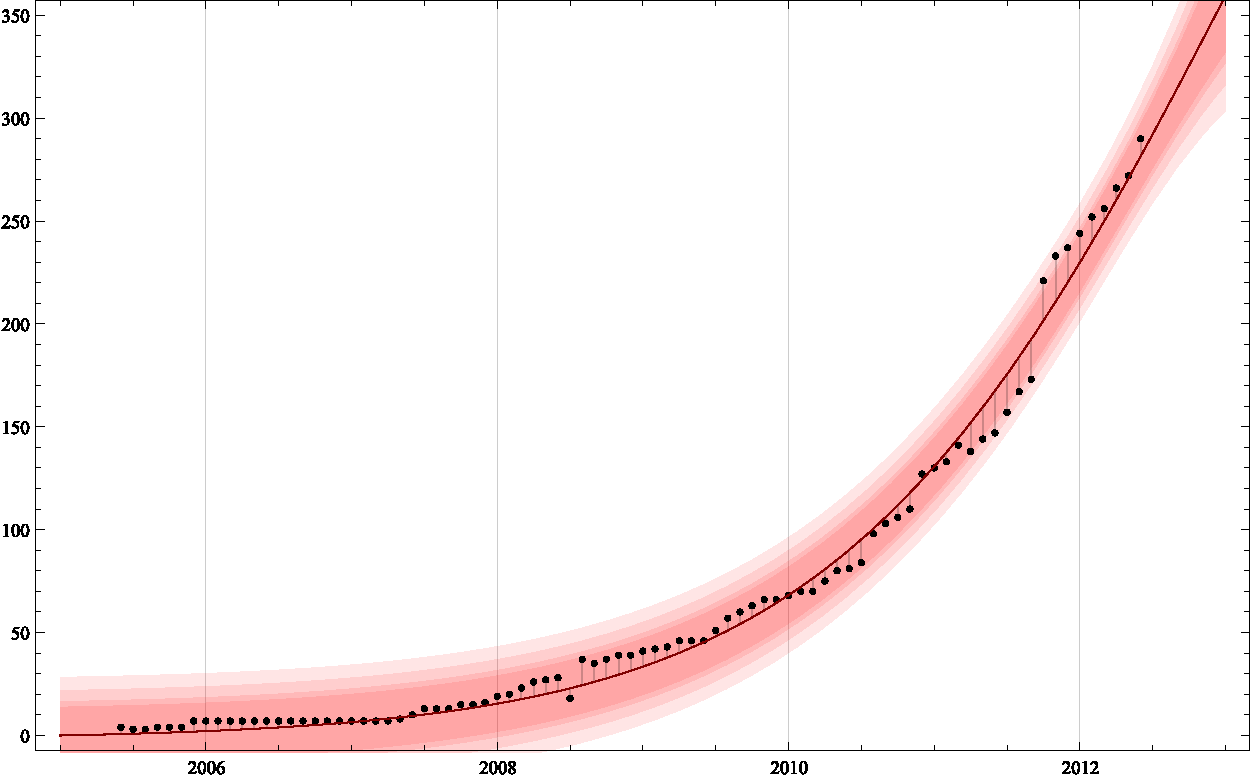
\includegraphics[width=\linewidth]{BassFit-git2.pdf}
\vspace{-2em}
\caption{The imitation driven adoption of \texttt{git}.}\label{fig:git}
\vspace{-1.5em}
\end{figure}

\subsection{Imitator Driven Growth}

The first package we consider is \verb|git|, a modern revision control system that shows an imitator driven adoption. It's growth can be seen in \ref{fig:git}, the corresponding statistics are in \ref{tbl:results}. The package first appeared just before 2005, it had around ten packages depending on it in 2006, twenty in 2008 and is currently used by almost three hundred packages. According to the Bass model, it will continue to grow to approximately 750 users. The innovator inflow is only $0.2\%$ of the potential market per year, so one would expect $0.002\cdot (750 - 300) = 1$ user to adopt \verb|git| out of sheer innovation. Taking the analogy with persons, if someone from the $450$ current non-users where to meet a random person from the entire $750$ market, there is a $\frac{300}{750}= 40\%$ chance of meeting a user which can convince him/her to start using \verb|git|. The chance of this happening is the imitator inflow $q = 0.73$. Therefore, the total number of users \verb|git| can expect to gain from imitation this year is $450\cdot 40\%\cdot 0.73 = 131$. Very much imitator driven!

The relative slowness of \verb|git|'s growth and its dependence on imitator can be explained. Open source projects, and software project in general, consist of numerous large textual files containing source code. Changes made in one place can hugely and unpredictably affect other places. To complicate matters further, usually more than one developer works on the source code at the same time. There are competing systems such as \verb|cvs|, \verb|subversion|, \verb|mercurial|, etcetera., but the basic functionality of maintaining version is provided by all of them. Thus two explanations can be derived for \verb|git|'s growth: First, the revision control system is not a part that affects the products delivered by the open source project and second, there is little incentive to switch unless the new revision control system is proved to be superior.

\verb|libnotify| is a library for notifications. In modern desktop environments applications may want to notify the user of certain events, for example a battery that is about to go empty, a new email or an incoming phone call. The adoption is relatively slow, despite its usefulness. A possible explanation is that the target applications all have their own custom solutions, which the developers are keen to keep.

\verb|udev| is a device manager. Its task is to communicate closely with the hardware drivers in Linux kernel to monitor any changes in the hardware configuration. It represents an architectural change in a very low level component, this might explain its slow imitator driven growth.

\verb|cairo| is a graphics library. It provides facilities for drawing lines, circles, text and other graphics primitives and is used by user graphics-heavy projects such as user interface libraries. Much like \verb|udev| it is an architectural change at a low level, this might explain its similar growth pattern.

\subsection{Innovator Driven Growth}

\begin{figure}
\centering
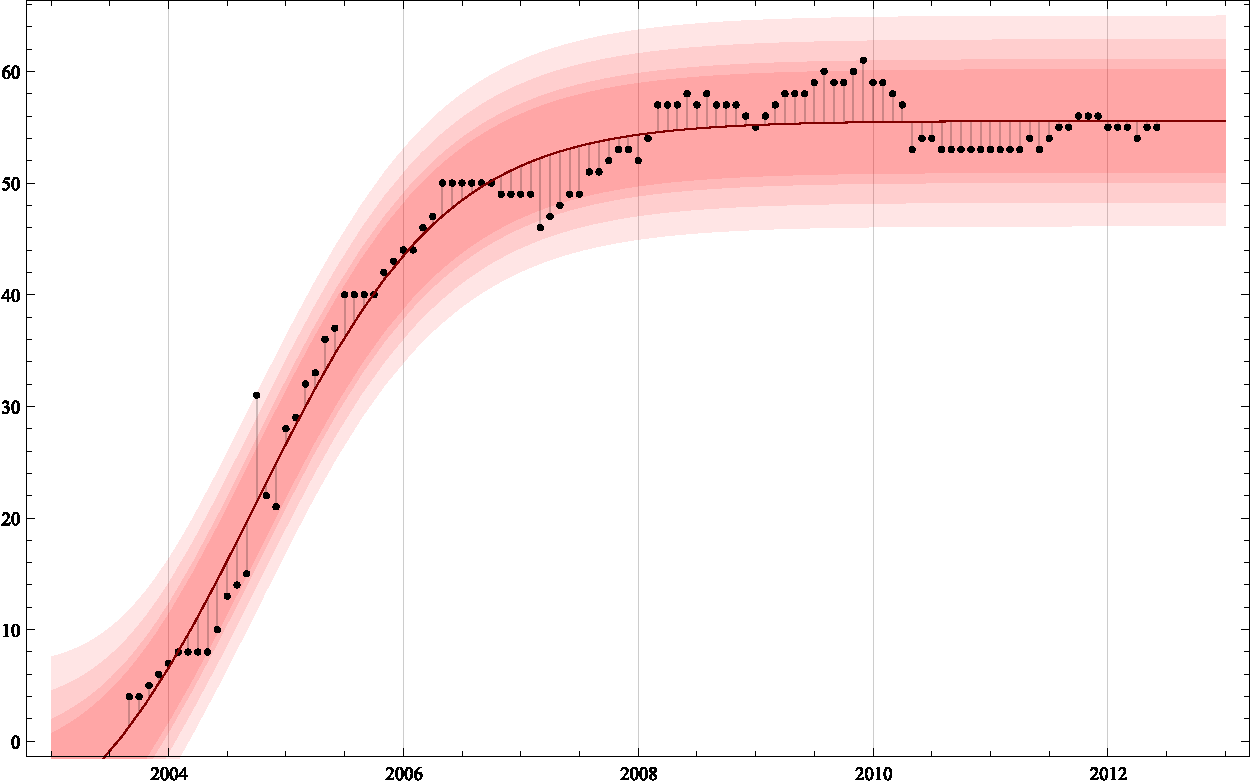
\includegraphics[width=\linewidth]{BassFit-libmad2.pdf}
\vspace{-2em}
\caption{The innovation driven adoption of \texttt{libmad}.}\label{fig:libmad}
\vspace{-1em}
\end{figure}

A typical example of innovator driven growth is given by \verb|libmad|. The model is fitted resulting in \ref{fig:libmad}. Again, the data is neatly explained by a Bass diffusion process, in particular the rapid steep growth and the stable user base afterwards. The name is an acronym for ``library for MPEG Audio Decoding'' and the package provides a high quality mp3 decoder for use in multimedia applications. This might also explain the rapid growth of its adoption: multimedia applications can benefit a lot from good quality mp3 support.

\verb|libtheora| is a library for the Schroedinger video codec. It implements a multimedia standard for use by video players. Just as with \verb|libmad| there is a strong innovator driven growth.

\verb|taglib| is a library that processes metadata from multimedia files. The package allows media players to read and store information such as artist and title from multimedia files. Again, like the other multimedia packages we observe rapid innovator driven growth.

\subsection{Growth and Demise}

\begin{figure}
\centering
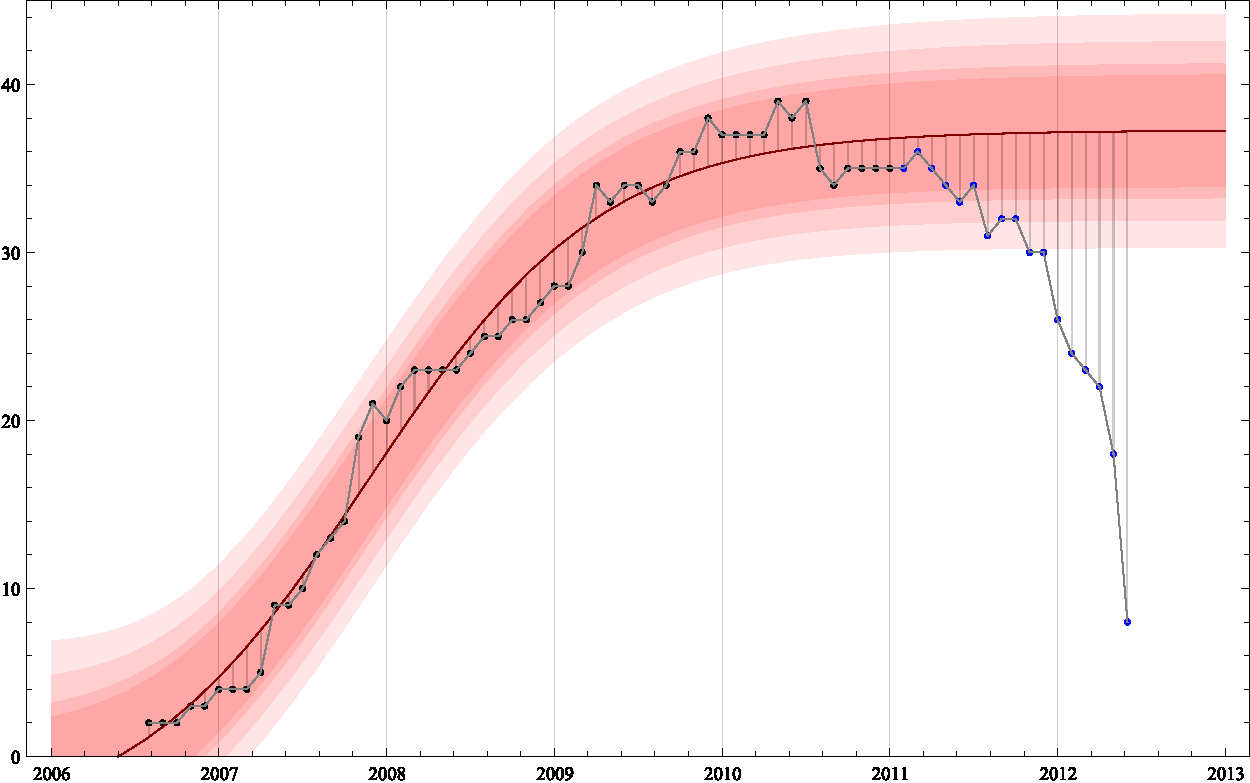
\includegraphics[width=\linewidth]{BassFit-xulrunner-22.pdf}
\vspace{-2em}
\caption{The rise and decline of \texttt{xulrunner}.}\label{fig:xulrunner}
\vspace{-1em}
\end{figure}

The previous examples are all about projects that start and undergo a growth phase that can be explained by a Bass diffusion process. So far, the Bass diffusion model has appeared to give a very accurate explanation of the adoption of an open source software library.

A Bass diffusion increases monotonically, and never declines. However, not all packages follow this behaviour. Project \verb|libmad| (see \ref{fig:libmad}) is a good example of this contra-behaviour. The package has an innovator driver growth that brings it close to its maximum in about two years. After that, the package's usage remains almost flat for years, and will do so indefinitely if it is a perfect Bass diffusion process. This is called the ``maturity stage'' in product life-cycle parlance.

A real product life-cycle will also include a ``decline stage'' where the product begins to become obsolete. The Bass innovation diffusion model does not account for this. In a deep sense it would not have to, once ideas spread they become part of our collective knowledge and will continue to be used by the new products being developed. But the Bass model was not developed for the spreading of ideas, it was developed in the context of marketing to model the adoption of products. Extending the Bass model to include obsolescence would be an interesting extension for future research.

The package \verb|xulrunner| in the dataset is a nice example of a short but complete life cycle, see \ref{fig:xulrunner}. When the Bass model is applied naively and a least mean squares best-fit is made, the result is a poor fit. If one looks at the dependency growth of the package, the cause is clear: the package becomes obsolete, which the Bass model as presented in section \ref{eq:bass} does not represent. The decline of the package from approximately 2011 onwards can be seen as blue dots in the figure.

Excluding the blue dots from the data results in the Bass model fit from figure \ref{fig:xulrunner}. The fitness increases to $\bar{R}^2=99.54\%$ and the parameters have tighter and reasonable confidence intervals. This is strong evidence that the initial adoption of the package is a Bass diffusion process. To explain the last part, the model should be extended with an obsolescence term. 


\subsection{Hypothesis testing}

· Filter on >2004  >30
· Select 10 randomly where
	· External confirmation that the project was actually started at that point in time and not as a spin-off or refactor.
	· No 'noise' Δ > 

Hypotheses: “Package dependency growth fits a Bass diffusion process”

To test this hypotheses we do the following: 

→ Explain why discontinuities are unnatural and filter on them

\begin{itemize}
	\item Start with all the packages in the Gentoo portage database. (21\,380)
	\item Filter out the packages that existed before 2004-01-01. (14\,706)
	\item Filter out packages that do not have at least 20 dependees at some point. (324)
	\item Filter out packages labeled “-virtual”, “-virtuals”, “-proto” or “-meta”. (259)
	\item Randomly pick packages and manually verify that:
	\begin{enumerate}
		\item[A.] The data does not contain strong discontinuities.
		\item[B.] The package corresponds to an open source project.
		\item[C.] The package has not been forked of or factored out of another package.
		\item[D.] The first included version should be close to a '1.0' release.
		\item[E.] That open source project has not been in Gentoo as (part of) some other package.
	\end{enumerate}
	This is verified by consulting
	\begin{itemize}
		\item The changelog of the ebuild
		\item Any readme or changelog included in the source code (earliest available version).
		\item The projects revision history.
		\item The projects homepage.
	\end{itemize}
\end{itemize}

\begin{table}
\caption{Rejected packages}\label{tbl:rejected}
\begin{tabular}{llll}
\toprule
Growth & Package & \multicolumn{2}{l}{Reason for excluding}\\
\midrule
\raisebox{-.15em}{
\includegraphics[height=.8em]{sparkline-173-app-arch-lzma-utils.pdf}} & \texttt{app-arch/lzma-utils} & C & (forked of LZMA SDK) \\
\raisebox{-.15em}{
\includegraphics[height=.8em]{sparkline-74-app-text-asciidoc.pdf}} & \texttt{app-text/asciidoc} & D & (first release in 2002) \\
\raisebox{-.15em}{
\includegraphics[height=.8em]{sparkline-23-app-text-sword-modules.pdf}} & \texttt{app-text/sword-modules} & A & (discontinuous  peak) \\
\raisebox{-.15em}{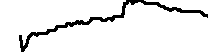
\includegraphics[height=.8em]{sparkline-35-dev-dotnet-gnome-sharp.pdf}} & \texttt{dev-dotnet/gnome-sharp} & A & (discontinuous jump) \\
\raisebox{-.15em}{
\includegraphics[height=.8em]{sparkline-166-dev-haskell-hscolour.pdf}} & \texttt{dev-haskell/hscolour} & D & (original release was in 2003) \\
\raisebox{-.15em}{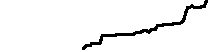
\includegraphics[height=.8em]{sparkline-159-dev-haskell-mtl.pdf}} & \texttt{dev-haskell/mtl} & C & (factored out of GHC) \\
\raisebox{-.15em}{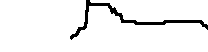
\includegraphics[height=.8em]{sparkline-146-dev-java-sun-jaf.pdf}} & \texttt{dev-java/sun-jaf} & B & (not open source) \\
\raisebox{-.15em}{
\includegraphics[height=.8em]{sparkline-39-dev-libs-liboil.pdf}} & \texttt{dev-libs/liboil} & A & (discontinuous  drop) \\
\raisebox{-.15em}{
\includegraphics[height=.8em]{sparkline-222-dev-php-pear.pdf}} & \texttt{dev-php/pear} & D & (first released in 2002) \\
\raisebox{-.15em}{
\includegraphics[height=.8em]{sparkline-150-dev-ruby-hoe.pdf}} & \texttt{dev-ruby/hoe} & A & (discontinuous  drop and jump) \\
\raisebox{-.15em}{
\includegraphics[height=.8em]{sparkline-51-dev-ruby-rake.pdf}} & \texttt{dev-ruby/rake} & A & (discontinuous  jump) \\
\raisebox{-.15em}{
\includegraphics[height=.8em]{sparkline-6-dev-util-cmake.pdf}} & \texttt{dev-util/cmake} & A & (discontinuous jump) \\
\raisebox{-.15em}{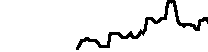
\includegraphics[height=.8em]{sparkline-198-dev-util-xfce4-dev-tools.pdf}} & \texttt{dev-util/xfce4-dev-tools} & C &(factored out of xfce) \\
\raisebox{-.15em}{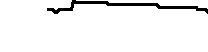
\includegraphics[height=.8em]{sparkline-122-games-fps-quake3-bin.pdf}} & \texttt{games-fps/quake3-bin} & B &(not open source) \\
\raisebox{-.15em}{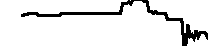
\includegraphics[height=.8em]{sparkline-60-kde-base-libkdepim.pdf}} & \texttt{kde-base/libkdepim} & C &(factored out of kdelibs) \\
\raisebox{-.15em}{
\includegraphics[height=.8em]{sparkline-221-kde-base-oxygen-icons.pdf}} & \texttt{kde-base/oxygen-icons} & C &(factored out of kdelibs) \\
\raisebox{-.15em}{
\includegraphics[height=.8em]{sparkline-152-mail-client-claws-mail.pdf}} & \texttt{mail-client/claws-mail} & C &(spun out of Sylpheed in 2001) \\
\raisebox{-.15em}{
\includegraphics[height=.8em]{sparkline-119-media-fonts-font-cursor-misc.pdf}} & \texttt{media-fonts/font-cursor-misc} & B & (not a software project) \\
\raisebox{-.15em}{
\includegraphics[height=.8em]{sparkline-79-media-libs-glew.pdf}} & \texttt{media-libs/glew} & D & (first released in 2002) \\
\raisebox{-.15em}{
\includegraphics[height=.8em]{sparkline-187-x11-libs-qt-phonon.pdf}} & \texttt{media-libs/phonon} & C &(factored out of kdelibs) \\
\raisebox{-.15em}{
\includegraphics[height=.8em]{sparkline-193-sys-apps-openrc.pdf}} & \texttt{sys-apps/openrc} & A & (discontinuous jump) \\
\raisebox{-.15em}{
\includegraphics[height=.8em]{sparkline-72-sys-apps-sandbox.pdf}} & \texttt{sys-apps/sandbox} & A &(discontinuous spike) \\
\raisebox{-.15em}{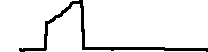
\includegraphics[height=.8em]{sparkline-48-sys-devel-automake-wrapper.pdf}} & \texttt{sys-devel/automake-wrapper} & B &(Gentoo logistical package) \\
\raisebox{-.15em}{
\includegraphics[height=.8em]{sparkline-199-x11-libs-libpciaccess.pdf}} & \texttt{x11-libs/libpciaccess} & A & (discontinuous jump) \\
\raisebox{-.15em}{
\includegraphics[height=.8em]{sparkline-109-x11-libs-libSM.pdf}} & \texttt{x11-libs/libSM} & C &(factored out of Xorg) \\
\raisebox{-.15em}{
\includegraphics[height=.8em]{sparkline-86-x11-libs-libXaw.pdf}} & \texttt{x11-libs/libXaw} & D &(originally from 1998) \\
\raisebox{-.15em}{
\includegraphics[height=.8em]{sparkline-104-x11-libs-libXdmcp.pdf}} & \texttt{x11-libs/libXdmcp} & C &(factored out of Xorg) \\
\raisebox{-.15em}{
\includegraphics[height=.8em]{sparkline-196-x11-libs-qt-demo.pdf}} & \texttt{x11-libs/qt-demo} & C &(factored out of Qt) \\
\raisebox{-.15em}{
\includegraphics[height=.8em]{sparkline-180-x11-libs-qt-opengl.pdf}} & \texttt{x11-libs/qt-opengl} & C &(factored out of Qt lib) \\
\raisebox{-.15em}{
\includegraphics[height=.8em]{sparkline-185-x11-libs-qt-script.pdf}} & \texttt{x11-libs/qt-script} & C &(factored out of Qt lib) \\
\bottomrule
\end{tabular}
\end{table}

\begin{table}
\caption{The ten selected packages}\label{tbl:selected}
\begin{tabular}{rlp{20em}}
\toprule
Growth & Package & Description \\
\midrule
\raisebox{-.15em}{
\includegraphics[height=.8em]{sparkline-34-dev-dotnet-gconf-sharp.pdf}} & \texttt{dev-dotnet/gconf-sharp} & GtkSharp's gconf module \\
\raisebox{-.15em}{
\includegraphics[height=.8em]{sparkline-65-dev-haskell-cabal.pdf}}  & \texttt{dev-haskell/cabal} & Framework for packaging Haskell software \\
\raisebox{-.15em}{
\includegraphics[height=.8em]{sparkline-218-dev-libs-libunique.pdf}}  & \texttt{dev-libs/libunique} & Library for writing single instance application \\
\raisebox{-.15em}{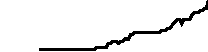
\includegraphics[height=.8em]{sparkline-77-dev-python-lxml.pdf}}  & \texttt{dev-python/lxml} & Python bindings for libxml2 and libxslt \\
\raisebox{-.15em}{
\includegraphics[height=.8em]{sparkline-157-dev-python-simplejson.pdf}}  & \texttt{dev-python/simplejson} & JSON encoder/decoder for Python \\
\raisebox{-.15em}{
\includegraphics[height=.8em]{sparkline-240-dev-vcs-git.pdf}}  & \texttt{dev-vcs/git} & The stupid content tracker \\
\raisebox{-.15em}{
\includegraphics[height=.8em]{sparkline-242-dev-vcs-mercurial.pdf}}  & \texttt{dev-vcs/mercurial} & Scalable distributed SCM \\
\raisebox{-.15em}{
\includegraphics[height=.8em]{sparkline-17-gnome-base-gnome-keyring.pdf}}  & \texttt{gnome-base/gnome-keyring} & Password and keyring managing daemon \\
\raisebox{-.15em}{
\includegraphics[height=.8em]{sparkline-206-media-libs-libcanberra.pdf}} & \texttt{media-libs/libcanberra} & Portable sound event library \\
\raisebox{-.15em}{
\includegraphics[height=.8em]{sparkline-143-x11-misc-xdg-utils.pdf}} & \texttt{x11-misc/xdg-utils} & Portland utils for interoperability \\
\bottomrule
\end{tabular}
\end{table}
% IDs = {34, 65, 218, 77, 157, 240, 242, 17, 206, 143}

% Initial values:
%  34: 12029/6,   20, 0.671, 0.131
%  65: 24067/12, 159, 0.061, 0.491
% 218: 24109/12,  37, 0.551, 0.141
%  77: 12031/6,   65, 0.011, 0.411
% 157: 24059/12, 104, 0.011, 0.421
% 240: 12031/6,  746, 0.000, 0.730
% 242: 2004,     159, 0.001, 0.621
%  17: 2004,      43, 0.021, 0.991
% 206: 8035/4,    37, 0.201, 0.961
% 143: 24083/12, 115, 0.041, 0.341

No packages where rejected on the 'E' ground, but many of these are covered by the 'C' reason. No extensive check was done on co-occurence of reasons.


XFree86 to XOrg. There are many packages (libFS, libSM, libICE, libWindowsWM, libX11, libXScrnsaver, etc..) that have been factored out of the X into separate libraries. All introduced in January 2006 and all having a version count starting at 1.0.0.

“The modern X.Org Foundation came into being in 2004 when the body that oversaw X standards and published the official reference implementation joined forces with former XFree86 developers. X11R6.7.0, the first version of the X.Org Server, was forked from XFree86 4.4 RC2. The immediate reason for the fork was a disagreement with the new license for the final release version of XFree86 4.4, but several disagreements among the contributors surfaced prior to the split. Many of the previous XFree86 developers have joined the X.Org Server project.”

“In 2005 a great effort was put in the modularization of the X.Org server source code,[18] resulting in a dual release by the end of the year. The X11R7.0.0 release added a new modular build system based on the GNU Autotools, while X11R6.9.0 release kept the old imake build system, both releases sharing the same codebase. Since then the X11R6.9 branch is maintained frozen and all the ongoing development is done to the modular (using GNU Autotools) branch. The new build system also brought the use of dlloader standard dynamic linker to load plugins and drivers, deprecating the old own method. As a consequence of the modularization, the X11 binaries were moving out of their own /usr/X11R6 subdirectory tree and into the global /usr tree on many Unix systems.”

More information about a packages can be found at
\begin{center}
\href{https://packages.gentoo.org/package/dev-vcs/git}{\texttt{https://packages.gentoo.org/package/\textcolor{MidnightBlue}{dev-vcs/git}}}
\end{center}
where \texttt{\textcolor{MidnightBlue}{dev-vcs/git}} is replaced with the name of the package.

The growth curves with large discontinuities are rejected. The hypotheses concerns open source projects depending on other open source projects. This is reflected in the Gentoo Portage dataset as dependency relations between packages, but this reflection can be quite noisy. It regularly happens that Gentoo developers re-organize the package database and within a datapoint (i.e. a single month) add or drop a large number of dependees to a package. The changes can be as large as a complete drop to zero or suddenly tripling the number of dependees. If this is translated back to dependee behaviour, it would mean that in a short span of time a large number of projects decide to use or drop a certain technology. Since the dependee projects are assumed to operate (mostly) independently, this is very unlikely. Even in instances of deprecation, where a project gets discontinued and tells its dependees to move on, the resulting decline is far from instantaneous. Therefore, growth curves with large discontinuities are rejected.


\begin{figure}
\centering
% 34, 65, 218, 77, 157, 240, 242, 17, 206, 143
\subfigure[\texttt{dev-dotnet/gconf-sharp}]{\includegraphics[width=0.45\textwidth]{BassFit-34-dev-dotnet-gconf-sharp.pdf}\label{fig:fit34}}
\subfigure[\texttt{dev-haskell/cabal}]{\includegraphics[width=0.45\textwidth]{BassFit-65-dev-haskell-cabal.pdf}\label{fig:fit65}}
\subfigure[\texttt{dev-libs/libunique}]{\includegraphics[width=0.45\textwidth]{BassFit-218-dev-libs-libunique.pdf}\label{fig:fit218}}
\subfigure[\texttt{dev-python/lxml}]{\includegraphics[width=0.45\textwidth]{BassFit-77-dev-python-lxml.pdf}\label{fig:fit77}}
\subfigure[\texttt{dev-python/simplejson}]{\includegraphics[width=0.45\textwidth]{BassFit-157-dev-python-simplejson.pdf}\label{fig:fit157}}
\subfigure[\texttt{dev-vcs/git}]{\includegraphics[width=0.45\textwidth]{BassFit-240-dev-vcs-git.pdf}\label{fig:fit240}}
\subfigure[\texttt{dev-vcs/mercurial}]{\includegraphics[width=0.45\textwidth]{BassFit-242-dev-vcs-mercurial.pdf}\label{fig:fit242}}
\subfigure[\texttt{gnome-base/gnome-keyring}]{\includegraphics[width=0.45\textwidth]{BassFit-17-gnome-base-gnome-keyring.pdf}\label{fig:fit17}}
\subfigure[\texttt{media-libs/libcanberra}]{\includegraphics[width=0.45\textwidth]{BassFit-206-media-libs-libcanberra.pdf}\label{fig:fit206}}
\subfigure[\texttt{x11-misc/xdg-utils}]{\includegraphics[width=0.45\textwidth]{BassFit-143-x11-misc-xdg-utils.pdf}\label{fig:fit143}}
\caption{Bass curve fits on ten randomly selected packages that met the criteria.}
\end{figure}



The package \texttt{dev-libs/libunique} does not have a good fit, but looking at the graph, \raisebox{-.15em}{\includegraphics[height=.8em,trim=7em 0 0 0,clip=true]{sparkline-218-dev-libs-libunique.pdf}}, it goes down at the end. This is demonstraded even more clearly in \texttt{net-libs/xulrunner}, \raisebox{-.15em}{\includegraphics[height=.8em,trim=3em 0 0 0,clip=true]{sparkline-140-net-libs-xulrunner.pdf}}, which declines almost completely.


\section{Conclusions and Future Work}

The growth of the number of packages depending on a packages can be modelled as a a Bass diffusion process. Overall the Bass diffusion model gave very a good fit for most OSS projects. Using only four parameters, it was able to describe the growth curves from the empirical data. Full statistical rigour would require a more involved analysis using the methods from, for example, \citet{carlos06}, but given the amount of and quality of evidence found we can conclude that most OSS project do follow the Bass diffusion model.

As can be seen in \ref{tbl:results}, the Bass parameters $p$ and $q$ are difficult to interpret and compare. A high $p$ does not automatically mean an innovator driven growth: if the $q$ value is also high then the result is simply a lot of growth. For the same reason it is also difficult to compare the $p$ and $q$ between packages. \citet{mahajan95} suggests using $\frac{q}{p}$ and $q + p$, this represents the total adoption rate and an imitator/innovator ratio.

Analysing the package dependency graph and its changes over time can provide new insights. Our exploratory study provides some evidence for insights such as how multimedia libraries are being adopted through an innovator driven process with low-level architectural changes happening slowly and through imitation. Further studies could test these hypotheses.

The package dependency graph contains empirical data to test extensions of the Bass diffusion model - extended with discarders. The Bass model and the present analysis is formulated in terms of absolute number of users, but in most applications only sales figures are available. The amount of sales is the first derivative of the Bass model, hence the model is usually applied in its derivative form \citep{mahajan95}. As a consequence the model only considers adopters, but does not consider \emph{discarders}. In the \verb|xulrunner| example, we see the package being discarded from 2011 onwards, providing insights in the discarding mechanism. The next step would be to collect more examples of packages being discard, look at their patterns of demise and develop a model of discarding to supplement the Bass model of adoption. One model could for example be the inverse of a Bass curve, this makes sense when the market share of the original package is taken over by a new package. The unique feature of dependency graph analysis to give absolute user numbers facilitates this. Such an analysis can also help in predicting the behaviour of certain projects - hence forewarning the particular project stakeholders.

The scale and complexity of the dependency graphs and open source innovation requires some care. Three notable issues became apparent in this study: First, In the open source community there is a lot of forking. It is not always clear whether a forked project constitutes the continuation of the original project or a separate new project. A more thorough study on the nature of forking could provide the insights to resolve this. Second, due to the public nature of open source development many immature or abandoned projects are visible in the larger datasets. This is good from a scientific perspective: it allows one to research projects from their early beginning and look at projects that failed to grow or became obsolete. But it clouds the `big picture' with many projects that do not significantly contribute to the overall innovation. In large datasets one would have to devise a relevance metric to select the relevant metrics. Such metrics could be the number of developers, the number users or the number of dependees. Third, the sheer scale of the available OSS databases provide challenges for analysis. Specialist tooling is required to transform the raw data into more manageable formats.

\section{Relevance — Implications to practice and research}

Type four theory: Explains and predicts.

\bibliographystyle{plainnat}
\bibliography{paper}
\end{document}
